\documentclass[11pt]{article}

% Compile with: tectonic qldpc_week1_week2_lecture_notes.tex
\usepackage[letterpaper,margin=0.82in]{geometry}
\usepackage[T1]{fontenc}
\usepackage{lmodern}
\usepackage{microtype}
\usepackage{mathtools,amssymb,bm}
\usepackage{booktabs,tabularx,longtable,array,multirow}
\usepackage[dvipsnames,table]{xcolor}
\usepackage{enumitem}
\usepackage{listings}
\usepackage{tikz}
\usetikzlibrary{arrows.meta,positioning,shapes.geometric,fit,calc,matrix}
\usepackage{quantikz}
\usepackage[most]{tcolorbox}
\usepackage{fancyhdr}
\usepackage{hyperref}

\definecolor{navy}{HTML}{17324D}
\definecolor{blue}{HTML}{2563EB}
\definecolor{teal}{HTML}{0F766E}
\definecolor{green}{HTML}{15803D}
\definecolor{amber}{HTML}{B45309}
\definecolor{red}{HTML}{B91C1C}
\definecolor{paper}{HTML}{F8FAFC}
\definecolor{line}{HTML}{CBD5E1}
\definecolor{ink}{HTML}{172033}
\definecolor{muted}{HTML}{52637A}

\hypersetup{
  colorlinks=true,
  linkcolor=blue,
  urlcolor=teal,
  citecolor=teal,
  pdftitle={qLDPC Foundations: Week 1 and Week 2 Lecture Notes},
  pdfauthor={QEC Research Project}
}

\pagestyle{fancy}
\fancyhf{}
\lhead{qLDPC CoDesign Explorer}
\rhead{Weeks 1--2 Learning Notes}
\cfoot{\thepage}
\setlength{\headheight}{14pt}
\renewcommand{\headrulewidth}{0.4pt}
\setlength{\parindent}{0pt}
\setlength{\parskip}{5pt}
\setlist{itemsep=2pt,topsep=4pt}

\newcommand{\Ftwo}{\mathbb{F}_2}
\providecommand{\ket}[1]{\lvert #1\rangle}
\providecommand{\bra}[1]{\langle #1\rvert}
\providecommand{\braket}[2]{\langle #1\mid #2\rangle}
\newcommand{\wt}{\operatorname{wt}}
\newcommand{\rank}{\operatorname{rank}}
\newcommand{\Span}{\operatorname{span}}

\newtcolorbox{learningbox}[1][]{
  enhanced,breakable,colback=blue!4,colframe=blue!75!black,
  boxrule=0.8pt,arc=2pt,title={Learning target},fonttitle=\bfseries,#1}
\newtcolorbox{conceptbox}[1][]{
  enhanced,breakable,colback=teal!4,colframe=teal!75!black,
  boxrule=0.8pt,arc=2pt,title={Core idea},fonttitle=\bfseries,#1}
\newtcolorbox{workedbox}[1][]{
  enhanced,breakable,colback=green!4,colframe=green!70!black,
  boxrule=0.8pt,arc=2pt,title={Worked example},fonttitle=\bfseries,#1}
\newtcolorbox{warningbox}[1][]{
  enhanced,breakable,colback=amber!5,colframe=amber!80!black,
  boxrule=0.8pt,arc=2pt,title={Common trap},fonttitle=\bfseries,#1}
\newtcolorbox{masterybox}[1][]{
  enhanced,breakable,colback=paper,colframe=navy,
  boxrule=1pt,arc=2pt,title={Mastery check},fonttitle=\bfseries,#1}
\newtcolorbox{hcibox}[1][]{
  enhanced,breakable,colback=violet!4,colframe=violet!70!black,
  boxrule=0.8pt,arc=2pt,title={HCI connection},fonttitle=\bfseries,#1}

\lstdefinestyle{python}{
  language=Python,
  basicstyle=\ttfamily\footnotesize,
  keywordstyle=\color{blue}\bfseries,
  commentstyle=\color{teal},
  stringstyle=\color{amber},
  showstringspaces=false,
  columns=fullflexible,
  keepspaces=true,
  frame=single,
  rulecolor=\color{line},
  backgroundcolor=\color{paper},
  breaklines=true,
  tabsize=4
}
\lstdefinestyle{json}{
  basicstyle=\ttfamily\footnotesize,
  showstringspaces=false,
  columns=fullflexible,
  keepspaces=true,
  frame=single,
  rulecolor=\color{line},
  backgroundcolor=\color{paper},
  breaklines=true
}

\title{\vspace{-1.8cm}\textbf{qLDPC Foundations}\\[3pt]
\Large Week 1 and Week 2 Lecture Notes and Guided Labs}
\author{qLDPC CoDesign Explorer}
\date{Start date: September 11, 2026}

\begin{document}
\maketitle

\begin{center}
\begin{minipage}{0.92\textwidth}
\small
These notes convert the first two weeks of the project plan into a teachable sequence. They are
written for a learner who knows basic linear algebra but is new to quantum error correction (QEC)
and quantum low-density parity-check (qLDPC) codes. The goal is operational understanding: you
should be able to calculate each object, explain what it means, and identify how it should appear in
the HCI prototype.
\end{minipage}
\end{center}

\tableofcontents
\newpage

\section{How to use these notes}

\begin{learningbox}
At the end of Week 1, you should be able to compute a classical syndrome, describe Pauli errors,
explain stabilizer measurements, and calculate separate CSS syndromes. At the end of Week 2, you
should be able to interpret \([[n,k,d]]\), read a Tanner graph, construct and validate a small HGP/CSS
fixture, explain BP--OSD at interface level, and map every technical state into a visible interaction.
\end{learningbox}

Because you are starting on Friday instead of Monday, call today \emph{Day 1}. Preserve the order of
the material; the concepts are cumulative. A workable schedule is:

\begin{center}
\begin{tabularx}{\textwidth}{>{\bfseries}p{0.10\textwidth}p{0.12\textwidth}X>{\raggedleft\arraybackslash}p{0.12\textwidth}}
\toprule
Day & Plan slot & Focus & Time \\
\midrule
1 & W1 Mon & Qubits, bases, and Pauli operators & 2.5 h \\
2 & W1 Tue & Binary codes, parity checks, and syndromes & 3 h \\
3 & W1 Wed & Stabilizers, commutation, and measurement & 3 h \\
4 & W1 Thu & CSS codes and separate error channels & 3 h \\
5 & W1 Fri & HCI charter, scope, and user journey & 2.5 h \\
6 & W2 Mon & \([[n,k,d]]\), degeneracy, LDPC, Tanner graphs & 3 h \\
7 & W2 Tue & Surface-code, HGP, and BB intuition & 3 h \\
8 & W2 Wed & Build and validate the \([[13,1,3]]\) fixture & 3 h \\
9 & W2 Thu & BP--OSD decoder spike and adapter contract & 3 h \\
10 & W2 Fri & Six-screen storyboard and interaction states & 3 h \\
\bottomrule
\end{tabularx}
\end{center}

For each day: (1) read the lesson, (2) reproduce every worked calculation without looking,
(3) complete the exercises, and (4) answer the ``say it aloud'' prompt. Do not treat recognition as
mastery. You understand a concept when you can calculate with it and explain it in plain language.

\begin{warningbox}
The project is an HCI learning and diagnostic tool, not a claim of a new qLDPC code or decoder.
Production UI work begins only after the syndrome exercises and scope gate are complete.
\end{warningbox}

\part{Week 1: QEC foundations and project framing}

\section{Day 1: Qubits, bases, and Pauli errors}

\subsection{A qubit is a normalized complex vector}

A pure qubit state is
\[
  \ket{\psi}=\alpha\ket{0}+\beta\ket{1}
  =\begin{bmatrix}\alpha\\\beta\end{bmatrix},
  \qquad \alpha,\beta\in\mathbb{C},
  \qquad |\alpha|^2+|\beta|^2=1.
\]
The computational basis vectors are
\[
  \ket{0}=\begin{bmatrix}1\\0\end{bmatrix},\qquad
  \ket{1}=\begin{bmatrix}0\\1\end{bmatrix}.
\]
A global phase is physically irrelevant: \(\ket{\psi}\) and \(e^{i\phi}\ket{\psi}\) describe the
same physical state. A relative phase is observable through interference.

The Hadamard or \(X\)-basis states are
\[
  \ket{+}=\frac{\ket{0}+\ket{1}}{\sqrt{2}},\qquad
  \ket{-}=\frac{\ket{0}-\ket{1}}{\sqrt{2}}.
\]
The Hadamard gate swaps the two bases:
\[
  H=\frac{1}{\sqrt{2}}\begin{bmatrix}1&1\\1&-1\end{bmatrix},
  \quad H\ket{0}=\ket{+},\quad H\ket{1}=\ket{-},\quad H^2=I.
\]

\subsection{The Pauli operators}

\[
I=\begin{bmatrix}1&0\\0&1\end{bmatrix},\quad
X=\begin{bmatrix}0&1\\1&0\end{bmatrix},\quad
Y=\begin{bmatrix}0&-i\\i&0\end{bmatrix},\quad
Z=\begin{bmatrix}1&0\\0&-1\end{bmatrix}.
\]

\begin{center}
\begin{tabular}{llll}
\toprule
Operator & Informal name & Computational-basis action & Hadamard-basis action \\
\midrule
\(X\) & bit flip & \(\ket{0}\leftrightarrow\ket{1}\) & \(\ket{+}\mapsto\ket{+}\), \(\ket{-}\mapsto-\ket{-}\) \\
\(Z\) & phase flip & \(\ket{0}\mapsto\ket{0}\), \(\ket{1}\mapsto-\ket{1}\) & \(\ket{+}\leftrightarrow\ket{-}\) \\
\(Y\) & bit and phase & \(\ket{0}\mapsto i\ket{1}\), \(\ket{1}\mapsto-i\ket{0}\) & both effects, up to phase \\
\bottomrule
\end{tabular}
\end{center}

Important algebra:
\[
X^2=Y^2=Z^2=I,\qquad XZ=-ZX,\qquad XY=iZ,\quad YZ=iX,\quad ZX=iY,
\qquad Y=iXZ.
\]
Thus distinct nonidentity Paulis anticommute. The sign or factor \(i\) often does not affect a
syndrome, but it matters in operator algebra.

\begin{workedbox}[title={Four state/error calculations}]
\textbf{1. Bit flip on \(\ket{0}\):}
\[
X\ket{0}=\begin{bmatrix}0&1\\1&0\end{bmatrix}
\begin{bmatrix}1\\0\end{bmatrix}=\begin{bmatrix}0\\1\end{bmatrix}=\ket{1}.
\]

\textbf{2. Phase flip on \(\ket{+}\):}
\[
Z\ket{+}=Z\frac{\ket{0}+\ket{1}}{\sqrt2}
=\frac{\ket{0}-\ket{1}}{\sqrt2}=\ket{-}.
\]

\textbf{3. Bit flip on \(\ket{-}\):}
\[
X\ket{-}=\frac{X\ket0-X\ket1}{\sqrt2}
=\frac{\ket1-\ket0}{\sqrt2}=-\ket{-}.
\]
The minus sign is a global phase, so the physical state is unchanged, but \(\ket{-}\) is an
eigenstate of \(X\) with eigenvalue \(-1\).

\textbf{4. \(Y\) error on \(\ket{+}\):}
\[
Y\ket{+}=iXZ\ket{+}=iX\ket{-}=-i\ket{-}.
\]
Up to global phase, \(Y\) changes \(\ket{+}\) to \(\ket{-}\).
\end{workedbox}

\subsection{Measurement and why the basis matters}

Measuring \(\ket{\psi}=\alpha\ket0+\beta\ket1\) in the computational basis returns 0 with
probability \(|\alpha|^2\) and 1 with probability \(|\beta|^2\). To measure in the \(X\) basis,
apply \(H\) and then measure in the computational basis.

\begin{center}
\begin{quantikz}[row sep=0.35cm,column sep=0.45cm]
\lstick{\(\ket{\psi}\)} & \gate{H} & \meter{} \rstick{\(X\)-basis result}
\end{quantikz}
\end{center}

This works because measuring \(H\ket\psi\) in the \(Z\) basis is equivalent to measuring
\(X=HZH\) on \(\ket\psi\).

\begin{masterybox}[title={Day 1 exercises}]
\begin{enumerate}
  \item Compute \(X\ket{+}\), \(Z\ket{-}\), \(Y\ket0\), and \(Y\ket1\).
  \item Show by matrix multiplication that \(XZ=-ZX\).
  \item A qubit is \((\ket0+i\ket1)/\sqrt2\). What are the probabilities of 0 and 1 in a
  computational-basis measurement?
  \item Explain aloud in 30 seconds: why can a \(Z\) error be invisible in a \(Z\)-basis
  measurement but visible after a Hadamard?
\end{enumerate}
\textbf{Answers:} (1) \(\ket+\), \(-\ket+\), \(i\ket1\), \(-i\ket0\). (2) The two products are
diagonal with opposite signs. (3) \(1/2\) and \(1/2\). (4) A \(Z\) error changes relative phase;
the Hadamard converts relative phase into a population difference.
\end{masterybox}

\section{Day 2: Binary linear codes, parity checks, and syndromes}

\subsection{Arithmetic over \(\Ftwo\)}

Binary error correction uses the field \(\Ftwo=\{0,1\}\). Addition and multiplication are modulo 2:
\[
1+1=0,\qquad 1-1=0,\qquad 1\cdot1=1.
\]
Addition is XOR. For vectors, every operation is componentwise modulo 2.

A binary linear \([n,k,d]\) code is a \(k\)-dimensional subspace of \(\Ftwo^n\). A parity-check
matrix \(H\in\Ftwo^{m\times n}\) defines the valid codewords:
\[
\mathcal C=\{c\in\Ftwo^n:Hc^T=0\}.
\]
If \(H\) has rank \(r\), then \(k=n-r\). Rows are parity checks; columns identify which checks
touch each bit.

If a valid word \(c\) experiences error \(e\), the received word is \(r=c+e\), and
\[
s=Hr^T=H(c+e)^T=Hc^T+He^T=He^T\pmod2.
\]
The syndrome \(s\) depends on the error, not on the encoded message.

\subsection{A running classical example}

Use the length-3 repetition code:
\[
H=\begin{bmatrix}1&1&0\\0&1&1\end{bmatrix}.
\]
Its constraints say \(c_1+c_2=0\) and \(c_2+c_3=0\), so
\(\mathcal C=\{000,111\}\).

\begin{workedbox}[title={Three hand-computed syndromes}]
\textbf{Error on bit 1:}
\[
e_1=\begin{bmatrix}1&0&0\end{bmatrix},\qquad
s_1=He_1^T=\begin{bmatrix}1\\0\end{bmatrix}.
\]

\textbf{Error on bit 2:}
\[
e_2=\begin{bmatrix}0&1&0\end{bmatrix},\qquad
s_2=He_2^T=\begin{bmatrix}1\\1\end{bmatrix}.
\]

\textbf{Error on bit 3:}
\[
e_3=\begin{bmatrix}0&0&1\end{bmatrix},\qquad
s_3=He_3^T=\begin{bmatrix}0\\1\end{bmatrix}.
\]
Notice the shortcut: the syndrome of a single-bit error at position \(j\) is column \(j\) of \(H\).
\end{workedbox}

\subsection{Sparsity and the Tanner graph}

The Hamming weight \(\wt(v)\) is the number of nonzero entries in \(v\). A sparse parity-check
matrix has few ones. Its Tanner graph is bipartite:

\begin{itemize}
  \item one variable node \(v_j\) for each column (bit or qubit),
  \item one check node \(c_i\) for each row,
  \item an edge \((c_i,v_j)\) exactly when \(H_{ij}=1\).
\end{itemize}

\begin{center}
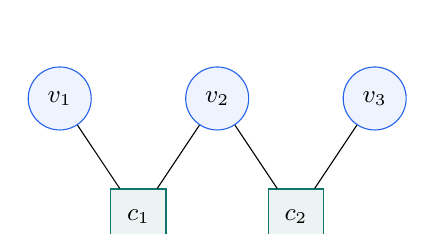
\begin{tikzpicture}[
  var/.style={circle,draw=blue,fill=blue!8,minimum size=8mm},
  chk/.style={rectangle,draw=teal,fill=teal!8,minimum size=7mm},
  every node/.style={font=\small}]
  \node[var] (v1) at (0,0) {\(v_1\)};
  \node[var] (v2) at (2,0) {\(v_2\)};
  \node[var] (v3) at (4,0) {\(v_3\)};
  \node[chk] (c1) at (1,-1.5) {\(c_1\)};
  \node[chk] (c2) at (3,-1.5) {\(c_2\)};
  \draw (v1)--(c1); \draw (v2)--(c1); \draw (v2)--(c2); \draw (v3)--(c2);
\end{tikzpicture}
\end{center}

Row weight is a check-node degree. Column weight is a variable-node degree. In an LDPC family,
these weights stay bounded as \(n\) grows. A single small matrix can be sparse, but the term LDPC
is fundamentally an asymptotic family property.

\subsection{Notebook-ready verification}

\begin{lstlisting}[style=python]
import numpy as np

H = np.array([[1, 1, 0],
              [0, 1, 1]], dtype=np.uint8)

examples = [
    (np.array([1, 0, 0], dtype=np.uint8), np.array([1, 0])),
    (np.array([0, 1, 0], dtype=np.uint8), np.array([1, 1])),
    (np.array([0, 0, 1], dtype=np.uint8), np.array([0, 1])),
]

for error, expected in examples:
    syndrome = (H @ error) % 2
    np.testing.assert_array_equal(syndrome, expected)
\end{lstlisting}

\begin{hcibox}
In the interface, selecting a matrix cell should highlight the corresponding Tanner-graph edge.
Injecting an error on variable \(v_j\) should highlight column \(j\), and every active check
\(s_i=1\) should receive the same visual status in the matrix, graph, and syndrome list.
\end{hcibox}

\begin{masterybox}[title={Day 2 exercises}]
For
\(
H'=\begin{bmatrix}1&1&0&1\\0&1&1&1\end{bmatrix}
\), calculate the syndromes of \(1000\), \(0100\), \(0010\), and \(1001\). Which two error
patterns have the same syndrome? What does that tell you?

\textbf{Answers:} \(10\), \(11\), \(01\), and \(01\), respectively. Thus \(0010\) and \(1001\)
have the same syndrome. Their difference \(1011\) is a codeword; a syndrome narrows the
possibilities but need not uniquely identify the physical error.
\end{masterybox}

\section{Day 3: Stabilizers, commutation, and syndrome measurement}

\subsection{The stabilizer viewpoint}

A Pauli operator \(S\) stabilizes \(\ket\psi\) if
\[
S\ket\psi=+\ket\psi.
\]
For example, \(Z\ket0=\ket0\) and \(X\ket+=\ket+\). A stabilizer code is the simultaneous
\(+1\) eigenspace of a commuting set of multi-qubit Pauli checks
\(S_1,\ldots,S_r\). Measuring \(S_i\) returns an eigenvalue \(m_i\in\{+1,-1\}\).
We encode it as a binary syndrome bit
\[
s_i=\frac{1-m_i}{2},
\]
so \(+1\mapsto0\) and \(-1\mapsto1\).

Suppose \(\ket\psi\) is in the code space and an error \(E\) occurs. If \(E\) commutes with
\(S_i\), then
\[
S_iE\ket\psi=ES_i\ket\psi=E\ket\psi,
\]
and the result remains \(+1\). If \(E\) anticommutes with \(S_i\), then
\[
S_iE\ket\psi=-ES_i\ket\psi=-E\ket\psi,
\]
so check \(i\) becomes active and returns \(-1\).

\begin{conceptbox}
A syndrome reports the pattern of checks that anticommute with the error. It does not directly
measure the logical amplitudes. QEC learns relational parity information about errors while leaving
the encoded state undisclosed.
\end{conceptbox}

\subsection{Fast commutation rules}

Two Pauli strings commute if the number of positions at which their single-qubit Paulis anticommute
is even; they anticommute if it is odd.

\begin{workedbox}[title={Commutation worksheet}]
\begin{center}
\begin{tabular}{lll}
\toprule
Pair & Local conflicts & Result \\
\midrule
\(XZI\) and \(ZII\) & qubit 1: \(X\) vs \(Z\), one conflict & anticommute \\
\(XXI\) and \(ZZI\) & qubits 1 and 2, two conflicts & commute \\
\(XYZ\) and \(ZYX\) & qubits 1 and 3, two conflicts & commute \\
\(XIZ\) and \(IIX\) & qubit 3: \(Z\) vs \(X\), one conflict & anticommute \\
\bottomrule
\end{tabular}
\end{center}
\end{workedbox}

\subsection{How an ancilla measures parity}

To measure a \(Z\)-type check such as \(Z_1Z_2Z_3\), prepare an ancilla in \(\ket0\), use each data
qubit as a CNOT control and the ancilla as target, then measure the ancilla. The data's computational
parity is copied to the ancilla without revealing the full data string.

\begin{center}
\begin{quantikz}[row sep=0.32cm,column sep=0.32cm]
\lstick{\(q_1\)} & \qw & \ctrl{3} & \qw      & \qw      & \qw \\
\lstick{\(q_2\)} & \qw & \qw      & \ctrl{2} & \qw      & \qw \\
\lstick{\(q_3\)} & \qw & \qw      & \qw      & \ctrl{1} & \qw \\
\lstick{\(a:\ket0\)} & \qw & \targ{} & \targ{} & \targ{} & \meter{}
\end{quantikz}
\end{center}

To measure an \(X\)-type check, prepare the ancilla in \(\ket+\), use it as the CNOT control onto the
data qubits, rotate it back with \(H\), and measure:

\begin{center}
\begin{quantikz}[row sep=0.32cm,column sep=0.32cm]
\lstick{\(a:\ket0\)} & \gate{H} & \ctrl{1} & \ctrl{2} & \ctrl{3} & \gate{H} & \meter{} \\
\lstick{\(q_1\)} & \qw & \targ{} & \qw & \qw & \qw & \qw \\
\lstick{\(q_2\)} & \qw & \qw & \targ{} & \qw & \qw & \qw \\
\lstick{\(q_3\)} & \qw & \qw & \qw & \targ{} & \qw & \qw
\end{quantikz}
\end{center}

These are idealized circuits. Fault-tolerant syndrome extraction requires careful ancilla design,
gate order, and repeated measurements. Those circuit-level details are outside this prototype's MVP,
which assumes perfect measurements and code-capacity noise.

\subsection{Plain-language explanation}

\begin{quote}\small
A QEC check asks a parity question about several physical qubits, rather than asking for the quantum
state stored in any one of them. Before an error, a valid encoded state has a known check value. An
error that anticommutes with a check flips that value, producing an active syndrome bit. Because the
check reveals only whether a relation is satisfied, it does not reveal the unknown logical amplitudes
being protected. Several errors may produce the same syndrome, so a decoder combines the syndrome
with a noise model to choose a likely correction. The correction does not need to match the physical
error exactly. It succeeds when error plus correction differs from identity only by a stabilizer; it
fails when their residual action is a nontrivial logical operator. In the interface, this causal chain
should remain visible: injected error, affected checks, proposed correction, residual syndrome, and
logical status must be distinct states.
\end{quote}

\begin{masterybox}[title={Day 3 exercises}]
Determine whether each error activates the check \(S=X_1X_2X_3X_4\):
\(Z_1\), \(Z_1Z_3\), \(X_2\), and \(Y_2Z_4\).

\textbf{Answers:} active, inactive, inactive, inactive. The last error has two local
anticommutations: \(Y\) vs \(X\) on qubit 2 and \(Z\) vs \(X\) on qubit 4.
\end{masterybox}

\section{Day 4: CSS codes and separate error channels}

\subsection{Binary representation of Pauli errors}

Ignoring global phase, represent an \(n\)-qubit Pauli error by two binary vectors:
\[
E\longleftrightarrow(e_X\mid e_Z)\in\Ftwo^{2n}.
\]
At qubit \(j\): \(I\leftrightarrow(0,0)\), \(X\leftrightarrow(1,0)\),
\(Z\leftrightarrow(0,1)\), and \(Y\leftrightarrow(1,1)\). Two Pauli vectors
\((x\mid z)\) and \((x'\mid z')\) commute exactly when their symplectic product vanishes:
\[
xz'^T+zx'^T=0\pmod2.
\]

\subsection{CSS structure}

A Calderbank--Shor--Steane (CSS) code separates its stabilizers into:
\begin{itemize}
  \item \(X\)-type checks described by \(H_X\), and
  \item \(Z\)-type checks described by \(H_Z\).
\end{itemize}
They commute when
\[
\boxed{H_XH_Z^T=0\pmod2.}
\]
With this notation, the syndromes are
\[
\boxed{s_Z=H_Ze_X^T},\qquad
\boxed{s_X=H_Xe_Z^T}.
\]
The subscript on \(s\) names the \emph{check type}, not the error type. Thus \(Z\)-checks detect
the \(X\) component, and \(X\)-checks detect the \(Z\) component. A \(Y\) error has both components
and can activate both channels.

If the check rows are independent within each type, the number of logical qubits is
\[
k=n-\rank_{\Ftwo}(H_X)-\rank_{\Ftwo}(H_Z).
\]
The rank formula remains correct with redundant rows as long as actual GF(2) ranks are used.

\subsection{A familiar CSS example: the Steane check matrix}

Let
\[
H_X=H_Z=H=
\begin{bmatrix}
1&0&1&0&1&0&1\\
0&1&1&0&0&1&1\\
0&0&0&1&1&1&1
\end{bmatrix}.
\]
Every row has even weight and every pair of distinct rows overlaps in an even number of positions,
so \(HH^T=0\). The matrix has rank 3, hence \(k=7-3-3=1\): this is a \([[7,1,3]]\) CSS code.

\begin{workedbox}[title={Two CSS syndrome calculations plus a \(Y\) check}]
\textbf{1. \(X\) error on qubit 5.} Here \(e_X=(0,0,0,0,1,0,0)\) and \(e_Z=0\). Therefore
\[
s_Z=H_Ze_X^T=\begin{bmatrix}1\\0\\1\end{bmatrix},\qquad s_X=0.
\]

\textbf{2. \(Z\) error on qubit 2.} Here \(e_Z=(0,1,0,0,0,0,0)\) and \(e_X=0\). Therefore
\[
s_X=H_Xe_Z^T=\begin{bmatrix}0\\1\\0\end{bmatrix},\qquad s_Z=0.
\]

\textbf{3. \(Y\) error on qubit 7.} Now \(e_X=e_Z=(0,0,0,0,0,0,1)\), so
\[
s_Z=s_X=\begin{bmatrix}1\\1\\1\end{bmatrix}.
\]
\end{workedbox}

\begin{warningbox}
Different texts swap the labels \(H_X\) and \(H_Z\). Always state your convention. These notes use
rows of \(H_X\) for \(X\)-type stabilizers and rows of \(H_Z\) for \(Z\)-type stabilizers.
\end{warningbox}

\begin{hcibox}
The UI should show two clearly labeled channels. Choosing \(X\) on qubit \(j\) updates
\(e_X\) and \(s_Z\); choosing \(Z\) updates \(e_Z\) and \(s_X\); choosing \(Y\) updates both.
This mapping should be visible in helper text, color-independent symbols, and the history log.
\end{hcibox}

\begin{masterybox}[title={Day 4 exercises}]
Using the Steane matrices above, calculate both syndrome vectors for
(a) \(X_3\), (b) \(Z_6\), and (c) \(Y_5\). Then verify one entry by counting local
anticommutations rather than multiplying matrices.

\textbf{Answers:} (a) \(s_Z=(1,1,0)^T,s_X=0\); (b)
\(s_X=(0,1,1)^T,s_Z=0\); (c) \(s_Z=s_X=(1,0,1)^T\).
\end{masterybox}

\section{Day 5: Project framing as an HCI system}

\subsection{Filled first-draft charter}

\begin{center}
\begin{tabularx}{\textwidth}{>{\bfseries\raggedright\arraybackslash}p{0.22\textwidth}X}
\toprule
Field & First-draft content \\
\midrule
Working title & qLDPC CoDesign Explorer \\
HCI question & How can coordinated visual representations and staged interaction make the causal
chain from code structure to physical error, syndrome, decoder correction, and hardware cost easier
to inspect and explain? \\
Primary audience & Students and quantum-computing learners with basic linear algebra but little
qLDPC experience; the instructor is the primary grading audience. \\
Core task & Configure one verified CSS qLDPC instance, inject a Pauli error, observe linked syndrome
representations, decode it, and inspect the correction and residual. \\
MVP evidence & A correct end-to-end scenario, deterministic fixtures, linked views, a usable staged
flow, inspection findings, tests, and honest limitations. \\
Noise boundary & Manual Pauli errors and seeded code-capacity sampling; perfect syndrome measurements. \\
Evaluation boundary & Expert inspection, task walkthroughs, accessibility checks, and correctness
tests; no claim of measured learning improvement and no required user study. \\
Explicit exclusions & New code design, neural decoding, multi-round or circuit-level noise, full
hardware routing, and production-grade decoder internals. \\
\bottomrule
\end{tabularx}
\end{center}

\subsection{Must, should, and could}

\begin{center}
\begin{tabularx}{\textwidth}{>{\bfseries\raggedright\arraybackslash}p{0.13\textwidth}X}
\toprule
Priority & Items \\
\midrule
Must & One verified HGP/CSS fixture; manual \(X/Z/Y\) injection; deterministic syndrome;
one decoder path; correction and residual; linked matrix/graph/state views; reset/undo; tests;
scope and limitation statements. \\
Should & Seeded code-capacity sampling; code-summary cards; observable decoder status and timing;
keyboard access; data-table fallback; simplified and transparent non-local-edge cost proxy. \\
Could & Additional BB example after the vertical-slice gate; richer animation; exportable scenario;
extra decoder comparison. \\
Will not in MVP & Neural decoder; arbitrary code synthesis; noisy measurement rounds;
circuit-level simulation; formal user study; full compiler or router. \\
\bottomrule
\end{tabularx}
\end{center}

\subsection{The learner's causal journey}

\begin{center}
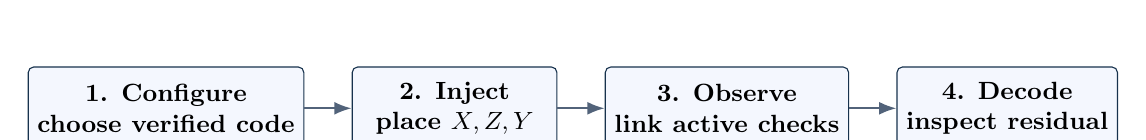
\begin{tikzpicture}[
  node distance=6mm,
  stage/.style={draw=navy,rounded corners=2pt,fill=blue!5,minimum width=2.6cm,
    minimum height=1.05cm,align=center,font=\small\bfseries},
  arrow/.style={-{Latex[length=2.2mm]},thick,draw=muted}]
\node[stage] (cfg) {1. Configure\\choose verified code};
\node[stage,right=of cfg] (inj) {2. Inject\\place \(X,Z,Y\)};
\node[stage,right=of inj] (obs) {3. Observe\\link active checks};
\node[stage,right=of obs] (dec) {4. Decode\\inspect residual};
\draw[arrow] (cfg)--(inj); \draw[arrow] (inj)--(obs); \draw[arrow] (obs)--(dec);
\end{tikzpicture}
\end{center}

The interface contribution is coordinated representation: a change in one view produces predictable,
consistent changes elsewhere. The matrix, Tanner graph, error vector, syndrome list, correction, and
history are different views of the same state, not separate demonstrations.

\begin{masterybox}[title={Week 1 pass condition}]
Without notes, take a small \(H\) and an \(X\) or \(Z\) error vector. Compute the active checks by
hand, reproduce the result with a GF(2) assertion, and point to every UI region that should change.
Then explain the distinction among error, syndrome, correction, and residual.
\end{masterybox}

\part{Week 2: qLDPC structure, decoding, and interaction design}

\section{Day 6: \texorpdfstring{\([[n,k,d]]\)}{[[n,k,d]]}, logical operators, degeneracy, and Tanner graphs}

\subsection{What \([[n,k,d]]\) means}

A quantum stabilizer code with parameters \([[n,k,d]]\) uses \(n\) physical qubits to encode
\(k\) logical qubits and has distance \(d\). The distance is the minimum weight of a Pauli operator
that commutes with every stabilizer but acts nontrivially on the logical subspace:
\[
d=\min\{\wt(P):P\in\mathcal N(\mathcal S)\setminus\mathcal S\},
\]
where \(\mathcal S\) is the stabilizer group and \(\mathcal N(\mathcal S)\) its Pauli normalizer.
The code can detect all errors of weight below \(d\) and correct arbitrary errors of weight
\(t=\lfloor(d-1)/2\rfloor\), assuming an ideal decoding model.

Logical Pauli operators \(\overline X_i,\overline Z_i\) commute with all stabilizers but are not
themselves stabilizers. They preserve the code space while changing encoded information.

\subsection{Degeneracy changes what ``correct'' means}

If errors \(E_1\) and \(E_2\) differ by a stabilizer, \(E_2=E_1S\), they act identically on every
code state. They also have the same syndrome. A quantum code is therefore degenerate: the decoder
should infer a likely \emph{equivalence class}, not necessarily the exact physical error.

Given true error \(e\) and proposed correction \(c\), define residual \(r=e+c\) in binary notation.
There are three useful levels of checking:
\begin{enumerate}
  \item \textbf{Syndrome consistency:} \(Hc^T=s\).
  \item \textbf{Zero residual syndrome:} \(Hr^T=0\).
  \item \textbf{Logical success:} the residual is a stabilizer, not a nontrivial logical operator.
\end{enumerate}
The first two do not by themselves prove logical success.

\subsection{What makes a quantum code LDPC?}

A CSS family is qLDPC if the row and column weights of both \(H_X\) and \(H_Z\) remain bounded as
the family grows. Operationally:
\begin{itemize}
  \item bounded row weight means every check touches only a bounded number of qubits;
  \item bounded column weight means every qubit participates in only a bounded number of checks;
  \item sparse Tanner graphs support local message passing such as belief propagation.
\end{itemize}
Low check weight does not imply geometric locality. A weight-6 check may couple six qubits that are
far apart in a planar device. Algebraic sparsity and hardware connectivity are distinct design axes.

\subsection{Code-summary card fields}

The Configure view should calculate rather than hard-code:
\[
n,\quad k,\quad \text{rate }k/n,\quad \rank(H_X),\quad\rank(H_Z),\quad
\max\text{ row weight},\quad\max\text{ column weight},\quad d\text{ if verified}.
\]
It should also name the construction, fixture version, provenance, qubit partition, and whether
distance is exact, bounded, or unknown.

\begin{masterybox}[title={Day 6 exercises}]
\begin{enumerate}
  \item How many arbitrary errors can a \([[13,1,3]]\) code correct in the ideal model?
  \item Why can two distinct corrections with the same syndrome have different logical outcomes?
  \item Explain why ``sparse matrix'' and ``easy hardware layout'' are not synonyms.
\end{enumerate}
\textbf{Answers:} (1) One. (2) Their difference has zero syndrome but may be either a stabilizer or
a logical operator. (3) Sparse checks have bounded degree, but their endpoints may still be far apart
on the physical connectivity graph.
\end{masterybox}

\section{Day 7: Surface codes, HGP codes, and bivariate bicycle codes}

\subsection{The surface-code reference point}

Surface codes place data qubits and local checks on a two-dimensional lattice. They have bounded
check weights, natural short-range layouts, and distance that grows with lattice linear size. Their
rate \(k/n\) tends to zero in the usual planar memory layouts. They are the hardware-local reference
point against which higher-rate qLDPC proposals are often compared.

\subsection{Hypergraph-product intuition}

The hypergraph product (HGP) turns two classical parity-check matrices
\(H_1\in\Ftwo^{m_1\times n_1}\) and \(H_2\in\Ftwo^{m_2\times n_2}\) into a CSS code:
\[
H_X=\left[H_1\otimes I_{n_2}\;\middle|\;I_{m_1}\otimes H_2^T\right],
\]
\[
H_Z=\left[I_{n_1}\otimes H_2\;\middle|\;H_1^T\otimes I_{m_2}\right].
\]
The physical qubits live in two sectors: \(n_1n_2\) vertex--vertex qubits and \(m_1m_2\)
check--check qubits, for
\[
n=n_1n_2+m_1m_2.
\]

Why do the checks commute? Multiply the blocks:
\[
H_XH_Z^T=(H_1\otimes H_2^T)+(H_1\otimes H_2^T)=0\pmod2.
\]
The same term appears twice and cancels over \(\Ftwo\). This is the central algebraic trick.

If the classical code dimensions are \(k_i=n_i-\rank(H_i)\) and the transpose-code dimensions are
\(k_i^T=m_i-\rank(H_i)\), then
\[
k=k_1k_2+k_1^Tk_2^T.
\]

\subsection{Bivariate bicycle intuition}

Bivariate bicycle (BB) codes are structured CSS qLDPC codes built from sparse polynomials in two
commuting cyclic-shift operators. In a common presentation, choose sparse commuting binary matrices
\(A\) and \(B\) and set
\[
H_X=[A\mid B],\qquad H_Z=[B^T\mid A^T].
\]
Then
\[
H_XH_Z^T=AB+BA=0\pmod2
\]
because \(A\) and \(B\) commute and the two identical binary terms cancel. The polynomial/circulant
structure can yield compact descriptions and useful code parameters, but a low-density algebraic
check does not guarantee short-range planar connectivity.

For this project, BB is a motivation and a later stretch example. The required MVP remains one
small, hand-verifiable HGP/CSS fixture. This prevents a sophisticated construction from hiding an
unverified causal chain.

\subsection{One-page comparison}

\small
\begin{longtable}{>{\bfseries\raggedright\arraybackslash}p{0.15\textwidth}
  >{\raggedright\arraybackslash}p{0.25\textwidth}
  >{\raggedright\arraybackslash}p{0.25\textwidth}
  >{\raggedright\arraybackslash}p{0.25\textwidth}}
\toprule
Dimension & Surface code & HGP code & BB code \\
\midrule
\endhead
Construction & Local cellulation/lattice with star and plaquette checks & Product of two classical
parity-check complexes & Sparse bivariate polynomials or commuting cyclic shifts \\
Check density & Bounded check and qubit degrees & Bounded when seed matrices have bounded degrees &
Bounded for sparse defining polynomials \\
Rate tendency & Usually vanishing in standard 2D planar families & Can approach a nonzero constant
for suitable seeds & Can encode multiple logical qubits with favorable finite-size overhead \\
Distance intuition & Set by shortest nontrivial path or loop & Inherited from seed-code and transpose-code
distances & Determined by algebraic structure; must be verified or bounded for a chosen instance \\
Connectivity & Naturally compatible with local 2D checks & Sparse but generally not planar-local &
Sparse but may require long-range or modular connections \\
Prototype role & Conceptual comparison, not the selected fixture & Required small verified MVP fixture &
Overview-level motivation; stretch only after the vertical slice \\
What the UI may claim & Shows the value of geometric locality & Demonstrates an inspectable product-built
CSS example & May describe published motivation and the selected fixture's verified facts only \\
\bottomrule
\end{longtable}
\normalsize

\begin{warningbox}
Do not turn broad literature claims into properties of the prototype. A published BB family, the
specific paper's fault-tolerant architecture, and this educational HGP fixture are three different
objects. Label construction facts, implementation choices, and future ideas separately.
\end{warningbox}

\begin{masterybox}[title={Day 7 say-it-aloud prompt}]
In two minutes, explain: (1) why HGP produces commuting CSS checks, (2) how BB uses commuting
shift structure, (3) why both may create hardware-connectivity challenges, and (4) why the MVP uses
the small HGP fixture rather than promising a full BB implementation.
\end{masterybox}

\section{Day 8: Construct and validate a small HGP/CSS fixture}

\subsection{Seed and resulting code}

Take the length-3 repetition-code check matrix twice:
\[
H_1=H_2=H=\begin{bmatrix}1&1&0\\0&1&1\end{bmatrix}.
\]
Here \(m=2,n=3,\rank(H)=2,k=1,k^T=0\). The HGP construction therefore has
\[
n=3\cdot3+2\cdot2=13,\qquad k=1\cdot1+0\cdot0=1.
\]
Brute-force verification gives distance 3, so the fixture is \([[13,1,3]]\).

The matrices have shape \(6\times13\):
\[
H_X=\left[H\otimes I_3\;\middle|\;I_2\otimes H^T\right],\qquad
H_Z=\left[I_3\otimes H\;\middle|\;H^T\otimes I_2\right].
\]
Their GF(2) ranks are both 6, all row weights are 3 or 4, and all column weights are at most 2.

\subsection{Reproducible construction and validation}

\begin{lstlisting}[style=python]
import itertools
import numpy as np

def gf2_rank(a):
    a = np.asarray(a, dtype=np.uint8).copy() % 2
    row = 0
    for col in range(a.shape[1]):
        pivots = np.flatnonzero(a[row:, col])
        if len(pivots) == 0:
            continue
        pivot = row + pivots[0]
        a[[row, pivot]] = a[[pivot, row]]
        for r in range(a.shape[0]):
            if r != row and a[r, col]:
                a[r] ^= a[row]
        row += 1
        if row == a.shape[0]:
            break
    return row

H = np.array([[1, 1, 0],
              [0, 1, 1]], dtype=np.uint8)
I3 = np.eye(3, dtype=np.uint8)
I2 = np.eye(2, dtype=np.uint8)

HX = np.concatenate([np.kron(H, I3), np.kron(I2, H.T)], axis=1) % 2
HZ = np.concatenate([np.kron(I3, H), np.kron(H.T, I2)], axis=1) % 2

assert HX.shape == (6, 13)
assert HZ.shape == (6, 13)
assert np.all((HX @ HZ.T) % 2 == 0)
assert gf2_rank(HX) == 6
assert gf2_rank(HZ) == 6
assert 13 - gf2_rank(HX) - gf2_rank(HZ) == 1
assert set(HX.sum(axis=1)).issubset({3, 4})
assert set(HZ.sum(axis=1)).issubset({3, 4})
assert HX.sum(axis=0).max() <= 2
assert HZ.sum(axis=0).max() <= 2

def row_space(A):
    values = set()
    for mask in range(1 << A.shape[0]):
        v = np.zeros(A.shape[1], dtype=np.uint8)
        for i in range(A.shape[0]):
            if (mask >> i) & 1:
                v ^= A[i]
        values.add(tuple(v.tolist()))
    return values

def min_css_logical(checks, same_type_stabilizers):
    stabilizers = row_space(same_type_stabilizers)
    for weight in range(1, checks.shape[1] + 1):
        for sites in itertools.combinations(range(checks.shape[1]), weight):
            v = np.zeros(checks.shape[1], dtype=np.uint8)
            v[list(sites)] = 1
            if np.all((checks @ v) % 2 == 0) and tuple(v.tolist()) not in stabilizers:
                return weight, sites
    raise RuntimeError("No logical operator found")

dX, logical_X_sites = min_css_logical(HZ, HX)
dZ, logical_Z_sites = min_css_logical(HX, HZ)
assert (dX, logical_X_sites) == (3, (0, 1, 2))
assert (dZ, logical_Z_sites) == (3, (0, 3, 6))
\end{lstlisting}

\subsection{Known-error scenarios}

For an \(X\) error on qubit 5,
\[
e_X=(0,0,0,0,1,0,0,0,0,0,0,0,0),
\qquad
s_Z=H_Ze_X^T=(0,0,1,1,0,0)^T.
\]
For a \(Z\) error on qubit 5,
\[
e_Z=(0,0,0,0,1,0,0,0,0,0,0,0,0),
\qquad
s_X=H_Xe_Z^T=(0,1,0,0,1,0)^T.
\]
For \(Y_5\), both syndrome patterns occur. These three scenarios are ideal deterministic fixtures for
the linked-view prototype.

One minimum-weight logical \(X\) representative is \(X_1X_2X_3\), and one minimum-weight logical
\(Z\) representative is \(Z_1Z_4Z_7\). Each has zero syndrome but is not a stabilizer. They make the
essential point that zero syndrome is not sufficient proof of logical success.

\subsection{Versioned fixture shape}

\begin{lstlisting}[style=json]
{
  "schema_version": 1,
  "fixture_id": "hgp_rep3_v1",
  "construction": "hypergraph_product",
  "parameters": {"n": 13, "k": 1, "d": 3, "distance_status": "verified"},
  "matrix_convention": {
    "HX": "rows are X-type checks; detects Z component",
    "HZ": "rows are Z-type checks; detects X component"
  },
  "noise_model": "code_capacity_perfect_measurement",
  "provenance": "HGP of two length-3 repetition parity-check matrices",
  "matrices": {"HX": "stored array", "HZ": "stored array"}
}
\end{lstlisting}

Validation should fail loudly if matrices are nonbinary, widths differ, orthogonality fails, declared
parameters disagree with computed ranks, or a golden syndrome changes.

\begin{masterybox}[title={Day 8 validation checklist}]
\begin{itemize}[label=\(\square\)]
  \item Reconstruct \(H_X,H_Z\) from \(H\) using Kronecker products.
  \item Assert both shapes, binary entries, and \(H_XH_Z^T=0\).
  \item Compute GF(2) ranks and derive \(k=1\).
  \item Check row and column weight distributions.
  \item Reproduce the \(X_5,Z_5,Y_5\) golden syndromes.
  \item Save arrays plus metadata under an immutable fixture identifier.
\end{itemize}
\end{masterybox}

\section{Day 9: Decoding and the BP--OSD spike}

\subsection{The decoding problem}

For one CSS channel, the decoder receives a binary parity-check matrix \(H\), a syndrome \(s\), and
a noise model. It returns a proposed correction \(c\) satisfying
\[
Hc^T=s.
\]
In this project:
\begin{itemize}
  \item decode the \(X\)-error component using \(H_Z\) and \(s_Z\);
  \item decode the \(Z\)-error component using \(H_X\) and \(s_X\);
  \item combine the two binary corrections into \(I/X/Z/Y\) labels.
\end{itemize}

\subsection{Belief propagation in one picture}

Belief propagation (BP) exchanges probabilistic messages along Tanner-graph edges:
\begin{enumerate}
  \item variable nodes begin with priors from the error channel;
  \item check nodes send messages expressing syndrome parity constraints;
  \item variable nodes combine incoming messages into updated beliefs;
  \item iteration stops on a syndrome-consistent estimate or at a limit.
\end{enumerate}
On a tree, the factorization is exact. qLDPC Tanner graphs contain cycles, so messages become
correlated and BP may fail to converge or may choose a poor representative, especially under
degeneracy.

Ordered statistics decoding (OSD) is a reliability-guided postprocessor. It uses BP reliabilities to
choose an information set, solves the syndrome constraint by binary elimination, and optionally tests
low-order flips among less reliable positions. BP supplies soft information; OSD supplies a robust
syndrome-consistent fallback.

\subsection{Current \texttt{ldpc} API spike}

The following is designed for \texttt{ldpc} 2.1.x and should be pinned and recorded in the notebook.
The package documentation states that \texttt{BpOsdDecoder.decode(syndrome)} returns a binary
correction and that BP--OSD falls back to OSD when BP does not converge.

\begin{lstlisting}[style=python]
# Record exact environment in the notebook:
# python -m pip install "ldpc==2.1.*"
import time
import numpy as np
import ldpc
from ldpc import BpOsdDecoder

def decode_channel(H, syndrome, error_rate=0.05):
    H = np.asarray(H, dtype=np.uint8)
    syndrome = np.asarray(syndrome, dtype=np.uint8)
    decoder = BpOsdDecoder(
        H,
        error_rate=error_rate,
        bp_method="product_sum",
        max_iter=max(20, H.shape[1]),
        schedule="serial",
        osd_method="osd_0",
        osd_order=0,
    )
    start = time.perf_counter()
    correction = np.asarray(decoder.decode(syndrome), dtype=np.uint8)
    elapsed_ms = 1000 * (time.perf_counter() - start)

    returned_syndrome = (H @ correction) % 2
    if not np.array_equal(returned_syndrome, syndrome):
        raise RuntimeError("Decoder returned a syndrome-inconsistent correction")

    return {
        "correction": correction,
        "syndrome_consistent": True,
        "bp_converged": bool(decoder.converge),
        "iterations": int(decoder.iter),
        "elapsed_ms": elapsed_ms,
    }

# X error on qubit 5: use HZ.
eX = np.zeros(13, dtype=np.uint8)
eX[4] = 1
sZ = (HZ @ eX) % 2
out_x = decode_channel(HZ, sZ)
residual_x = eX ^ out_x["correction"]
assert np.all((HZ @ residual_x) % 2 == 0)

# Z error on qubit 5: use HX.
eZ = np.zeros(13, dtype=np.uint8)
eZ[4] = 1
sX = (HX @ eZ) % 2
out_z = decode_channel(HX, sX)
residual_z = eZ ^ out_z["correction"]
assert np.all((HX @ residual_z) % 2 == 0)

print(ldpc.__version__, out_x, out_z)
\end{lstlisting}

\begin{warningbox}
\texttt{decoder.converge} reports whether the BP stage converged; it is not the same as logical
success. Always compute returned syndrome and residual. For a full logical-success test, reduce the
residual modulo the appropriate stabilizer row space and check logical equivalence.
\end{warningbox}

\subsection{Adapter decision and fallback}

The UI should depend on a small stable adapter, not on library-specific objects:

\begin{center}
\begin{tabularx}{\textwidth}{>{\ttfamily\raggedright\arraybackslash}p{0.26\textwidth}X}
\toprule
Adapter field & Meaning \\
\midrule
channel & \texttt{x} or \texttt{z}; states which error component is being decoded \\
input\_syndrome & exact binary syndrome sent to the decoder \\
correction & binary vector returned by the backend \\
residual & true fixture error XOR correction, available in prescribed demonstrations \\
syndrome\_consistent & whether \(Hc^T=s\) \\
residual\_syndrome & \(H(e+c)^T\) \\
status & completed, failed, invalid-input, or timeout \\
bp\_converged & observable BP flag if exposed \\
iterations, elapsed\_ms & observable performance fields if exposed \\
backend, version, settings & reproducibility metadata \\
\bottomrule
\end{tabularx}
\end{center}

If installation or API integration exceeds four hours, use an exact lookup or minimum-weight decoder
for the tiny fixture. Label it honestly. The HCI narrative requires an inspectable input--output chain,
not a particular decoder brand.

\begin{masterybox}[title={Day 9 decoder checks}]
For one \(X\) error and one \(Z\) error, record: input check matrix, syndrome, prior error rate,
correction, returned syndrome, residual, residual syndrome, convergence flag, iterations, runtime,
package version, and settings. Explain why a syndrome-consistent correction can still be a logical
failure.
\end{masterybox}

\section{Day 10: Turn technical states into a six-screen storyboard}

\subsection{The interaction contract}

Every screen should answer three questions: \emph{Where am I? What changed? What can I do next?}
The four conceptual stages become six concrete screens because configuration and decoding each need a
distinct result state.

\small
\begingroup
\setlength{\tabcolsep}{4pt}
\begin{longtable}{>{\bfseries\raggedright\arraybackslash}p{0.05\textwidth}
  >{\raggedright\arraybackslash}p{0.14\textwidth}
  >{\raggedright\arraybackslash}p{0.21\textwidth}
  >{\raggedright\arraybackslash}p{0.25\textwidth}
  >{\raggedright\arraybackslash}p{0.25\textwidth}}
\toprule
No. & Screen & System state & Visible representations & Primary action and feedback \\
\midrule
\endhead
1 & Welcome / empty & No fixture loaded & Four-stage stepper, short purpose, sample-code choice &
Load verified example; disable later stages with explanation \\
2 & Configured & Fixture valid & \([[n,k,d]]\) card, \(H_X/H_Z\), Tanner graph, provenance, model boundary &
Select matrix row/column; linked highlight; continue to Inject \\
3 & Inject & Editable Pauli vector & Qubit map, \(e_X/e_Z\), current error weight, history &
Place \(X/Z/Y\); undo/reset; invalid actions produce local error text \\
4 & Observe & Syndrome computed & Active checks in matrix, Tanner graph, and syndrome list; causal explanation &
Select an active check; all linked views highlight the same IDs \\
5 & Decode / loading & Request in flight & Frozen input summary, progress/status region, cancel or retry policy &
Run decoder; announce loading accessibly; prevent duplicate requests \\
6 & Decode / result & Correction available & Correction, residual, syndrome consistency, BP status, iterations, timing, limitations &
Compare error/correction; restart, change error, or inspect co-design metric \\
\bottomrule
\end{longtable}
\endgroup
\normalsize

\subsection{Single source of truth}

The interaction state can be described as
\[
\texttt{AppState}=(\texttt{fixture},\texttt{selection},e_X,e_Z,s_X,s_Z,
\texttt{decoderRun},\texttt{history}).
\]
Matrix color, Tanner-node status, cards, and explanation text are derived views. They must not carry
independent copies of the syndrome or selection.

Recommended state transitions:
\[
\texttt{empty}\to\texttt{configured}\to\texttt{injected}\to
\texttt{observed}\to\texttt{decoding}\to\texttt{decoded}.
\]
Changing the fixture resets all downstream data. Changing an error invalidates the old syndrome and
decoder result. Undo restores the prior complete state rather than only repainting the current view.

\subsection{Selection linking and visual language}

Use stable semantic identifiers such as \texttt{qubit:5}, \texttt{x-check:2}, and
\texttt{z-check:4}. A selection event identifies an entity; each view decides how to render it.
Never make color the only carrier of meaning. Combine color with icons, outlines, labels, and a
data-table representation.

\begin{center}
\begin{tabular}{lll}
\toprule
Semantic state & Suggested redundant encoding & Meaning \\
\midrule
selected & blue outline + focus ring & current object of inspection \\
error & amber \(\times\) marker + Pauli letter & injected physical error \\
active check & red filled square + ``1'' label & violated stabilizer check \\
correction & teal hatch + tool icon & decoder proposal \\
residual clear & green check + ``0 syndrome'' & no remaining detected violation \\
unknown/limited & gray dashed border + text & unavailable or intentionally omitted \\
\bottomrule
\end{tabular}
\end{center}

\subsection{Empty, loading, error, and recovery states}

\begin{itemize}
  \item \textbf{Empty:} explain why no data is shown and offer the verified fixture.
  \item \textbf{Loading:} preserve the submitted syndrome, show status, and announce progress.
  \item \textbf{Invalid input:} name the violated constraint and keep the user's recoverable work.
  \item \textbf{Decoder failure:} distinguish timeout, backend error, and inconsistent output; offer retry
  or the documented fallback.
  \item \textbf{Undo/reset:} undo one semantic action; reset asks for confirmation only if meaningful
  work would be lost.
\end{itemize}

\begin{hcibox}
Progressive disclosure is the central rationale. The learner first chooses a trustworthy code, then
manipulates an error, then sees its consequences, then asks for a correction. Showing every matrix,
metric, and decoder detail at once would obscure this causal order.
\end{hcibox}

\begin{masterybox}[title={Week 2 pass condition}]
One command must load the fixture, validate \(H_XH_Z^T=0\), inject a known error, compute the
expected syndrome, call the decoder, and verify the residual. The storyboard must show the identical
fixture ID, error, syndrome, correction, and residual across all relevant screens.
\end{masterybox}

\part{Consolidation and reference}

\section{End-to-end mental model}

\begin{center}
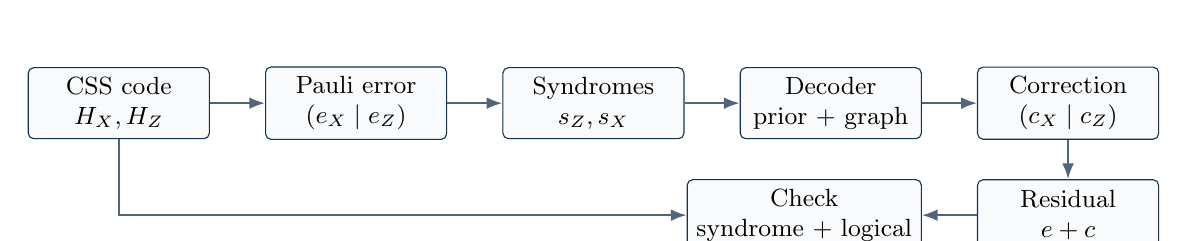
\begin{tikzpicture}[
  node distance=5mm and 7mm,
  box/.style={draw=navy,rounded corners=2pt,fill=paper,minimum height=9mm,
    minimum width=2.3cm,align=center,font=\small},
  arr/.style={-{Latex[length=2mm]},thick,draw=muted}]
\node[box] (code) {CSS code\\\(H_X,H_Z\)};
\node[box,right=of code] (err) {Pauli error\\\((e_X\mid e_Z)\)};
\node[box,right=of err] (syn) {Syndromes\\\(s_Z,s_X\)};
\node[box,right=of syn] (dec) {Decoder\\prior + graph};
\node[box,right=of dec] (corr) {Correction\\\((c_X\mid c_Z)\)};
\node[box,below=of corr] (res) {Residual\\\(e+c\)};
\node[box,left=of res] (judge) {Check\\syndrome + logical};
\draw[arr] (code)--(err); \draw[arr] (err)--(syn); \draw[arr] (syn)--(dec);
\draw[arr] (dec)--(corr); \draw[arr] (corr)--(res); \draw[arr] (res)--(judge);
\draw[arr] (code.south) |- (judge.west);
\end{tikzpicture}
\end{center}

\begin{enumerate}
  \item \(H_X,H_Z\) define commuting stabilizer checks and the code space.
  \item A Pauli error becomes two binary components \((e_X\mid e_Z)\).
  \item Cross-type checks expose it: \(s_Z=H_Ze_X^T\), \(s_X=H_Xe_Z^T\).
  \item A decoder uses the sparse graph and a noise prior to propose a syndrome-consistent correction.
  \item The residual determines success: zero syndrome is necessary, and stabilizer equivalence is the
  stronger logical criterion.
  \item The HCI system makes each transition visible while keeping the representations synchronized.
\end{enumerate}

\section{Notation glossary}

\begin{longtable}{>{\bfseries}p{0.18\textwidth}p{0.72\textwidth}}
\toprule
Symbol or term & Meaning \\
\midrule
\endhead
\(\Ftwo\) & Binary field with addition and multiplication modulo 2 \\
\(\wt(v)\) & Hamming weight: number of nonzero entries \\
\([n,k,d]\) & Classical code length, dimension, and distance \\
\([[n,k,d]]\) & Quantum code physical qubits, logical qubits, and distance \\
\(H\) & Classical parity-check matrix \\
\(H_X,H_Z\) & CSS matrices whose rows represent \(X\)-type and \(Z\)-type checks \\
\(e_X,e_Z\) & Binary vectors for the \(X\) and \(Z\) components of a Pauli error \\
\(s_X,s_Z\) & Outcomes of \(X\)-type and \(Z\)-type checks \\
syndrome & Binary pattern of violated checks \\
stabilizer & Pauli operator that fixes every code state \\
logical operator & Pauli that preserves the code space but acts nontrivially within it \\
normalizer & Paulis that commute with the stabilizer group \\
degeneracy & Distinct physical errors differing by a stabilizer have the same logical action \\
CSS code & Stabilizer code with separate \(X\)-type and \(Z\)-type checks \\
LDPC & Code family with bounded parity-check row and column weights \\
Tanner graph & Bipartite graph connecting variables/qubits to parity checks \\
HGP & Hypergraph-product construction that combines two classical parity-check complexes \\
BB code & Bivariate bicycle code built from sparse commuting cyclic-shift structure \\
BP & Belief propagation: iterative message passing on a Tanner graph \\
OSD & Ordered statistics decoding: reliability-guided algebraic postprocessing \\
correction & Decoder's proposed Pauli operation \\
residual & Error composed with correction; XOR in the binary representation \\
code-capacity noise & Data-qubit errors with ideal syndrome measurements \\
\bottomrule
\end{longtable}

\section{Final self-test}

Complete this without notes.

\begin{enumerate}
  \item Explain the physical difference between \(X\), \(Z\), and \(Y\).
  \item Given a binary matrix and error vector, compute \(He^T\bmod2\).
  \item Decide whether two Pauli strings commute using local anticommutation count.
  \item Explain why a stabilizer measurement does not reveal logical amplitudes.
  \item State the CSS orthogonality condition and both syndrome equations using the convention in
  these notes.
  \item Explain \([[n,k,d]]\), degeneracy, and the difference between zero residual syndrome and
  logical success.
  \item Draw the Tanner graph of a small matrix and derive row/column weights from it.
  \item Derive the HGP block matrices and explain why their product vanishes.
  \item Compare surface, HGP, and BB codes without confusing literature facts with prototype features.
  \item Validate the \([[13,1,3]]\) fixture and reproduce the \(X_5,Z_5,Y_5\) syndromes.
  \item Explain what BP contributes, what OSD contributes, and what decoder observables the UI may show.
  \item Walk through the six screens and name what changes in every linked representation.
\end{enumerate}

If any answer requires memorized wording, return to the corresponding worked example and perform a
new calculation with a different qubit or check.

\section{Two-minute verbal checkpoint script}

Use this only after attempting an explanation without notes:

\begin{quote}\small
The prototype begins with a verified CSS code represented by two sparse binary matrices. Rows are
stabilizer checks, columns are physical qubits, and matrix ones become Tanner-graph edges. A Pauli
error is split into binary \(X\) and \(Z\) components. Because unlike Paulis anticommute, \(Z\)-type
checks detect the \(X\) component and \(X\)-type checks detect the \(Z\) component. Their binary
matrix products form the syndrome. A decoder uses that syndrome and a noise prior to propose a
correction. It need not identify the exact physical error because errors that differ by a stabilizer
are equivalent. We first verify that the correction has the requested syndrome and that the residual
has zero syndrome, then distinguish this from the stronger condition of logical success. qLDPC means
that check and qubit degrees remain bounded across a code family, although sparse algebra does not
guarantee local hardware connections. The HCI contribution is a staged Configure--Inject--Observe--
Decode workflow whose matrix, graph, vectors, history, decoder result, and limitations remain visibly
synchronized.
\end{quote}

\section{Sources and further reading}

\begin{thebibliography}{9}
\bibitem{plan}
\emph{qLDPC CoDesign Explorer: 10-Week Project Plan}, Sections 6--7, local project document, 2026.

\bibitem{tutorial}
D. J. Spencer et al., \emph{Quantum error correction and fault tolerance: A comprehensive tutorial},
arXiv:2605.29137, 2026. Local copy: \texttt{Research Papers/QEC tutorial.pdf}.

\bibitem{gottesman}
D. Gottesman, \emph{Stabilizer Codes and Quantum Error Correction}, Ph.D. thesis,
California Institute of Technology, 1997, arXiv:quant-ph/9705052.

\bibitem{hgp}
J.-P. Tillich and G. Z\'emor, ``Quantum LDPC codes with positive rate and minimum distance
proportional to the square root of the blocklength,'' \emph{IEEE Transactions on Information Theory},
vol. 60, no. 2, 2014.

\bibitem{bb}
S. Bravyi et al., ``High-threshold and low-overhead fault-tolerant quantum memory,''
\emph{Nature}, vol. 627, 2024.

\bibitem{gross}
T. J. Yoder et al., \emph{Tour de gross: A modular quantum computer based on bivariate bicycle
codes}, arXiv:2506.03094, 2025. Local project copy.

\bibitem{ldpcdocs}
J. Roffe et al., \emph{LDPC documentation}, version 2.1.0,
\url{https://software.roffe.eu/ldpc/quantum_decoder.html}, accessed September 11, 2026.
\end{thebibliography}

\appendix
\section{Instructor checkpoint questions}

\begin{enumerate}
  \item Is one end-to-end qLDPC example sufficient for the course's technical bar?
  \item Does the four-stage interaction make the HCI contribution clear without a user study?
  \item Which final artifacts are mandatory: report, poster, video, live demo, or source code?
  \item Is the \([[13,1,3]]\) HGP fixture acceptable as the graded MVP while BB remains stretch scope?
  \item Is inspection plus deterministic task walkthrough and correctness testing sufficient evidence
  under the course rubric?
\end{enumerate}

\section{Deliverable checklist for Weeks 1 and 2}

\begin{itemize}[label=\(\square\)]
  \item One-page notation glossary and four solved state/error examples.
  \item Three hand-computed classical syndromes reproduced with assertions.
  \item Commutation worksheet and plain-language explanation.
  \item Two CSS syndrome calculations and an orthogonality assertion.
  \item One-page project charter and MVP/stretch backlog.
  \item Matrix-to-Tanner exercise and code-summary fields.
  \item Surface/HGP/BB comparison with facts separated from prototype features.
  \item Versioned \([[13,1,3]]\) JSON/NPZ fixture and validation tests.
  \item BP--OSD notebook spike, stable adapter decision, and fallback note.
  \item Six-screen storyboard and interaction-state table.
\end{itemize}

\end{document}
